% \chapter{RESTRAINT MOMENTS}
\chapter{约束弯矩}
% This appendix provides methods of estimating the restraining moment developed in prestressed girders when girders are made continuous over supports, as well as methods to mitigate the problem.
本附录提供了当梁在支撑上连续制作时预应力梁产生的约束弯矩的估算方法,以及减轻该问题的方法。
% \section{BACKGROUND}
\section{背景}
% In simple-span non-composite bridges, time-dependent deformations result in little or no change in the distribution of forces and moments within the structure. However, continuous multiple-span composite bridges are statically indeterminate. As a result, inelastic deformations that occur following construction will generally induce statically indeterminate forces and restraining moments in the girders.
在简支的非组合桥梁中,随时间变化的变形导致结构内力和力矩重分布的变化很小,或根本没有变化。然而,连续的多跨组合桥是超静定的,因此,施工后发生的非弹性变形通常会在梁中引起超静定力和约束力矩。

% Sources of inelastic deformation include concrete creep and shrinkage, and temperature gradients. For example, a common type of jointless bridge construction consists of precast, prestressed girders connected with a continuous cast-in-place deck slab as illustrated in \cref{fig:sdlc-beam}. The girders are simply supported for dead load but may be considered continuous for live load. Continuity is established with deck steel as negative moment reinforcement over the piers. Commonly, a positive moment connection is also provided in the diaphragms.
产生非弹性变形的根源包括混凝土徐变和收缩以及温度梯度。例如,一种常见的无缝桥梁结构由预制预应力梁与连续现浇桥面板连接而成,如\cref{fig:sdlc-beam} 所示。主梁仅受恒载,但对于活载可认为是连续的。 连续性是用甲板钢作为桥墩上的负力矩钢筋建立的。 通常,横隔梁中还提供正力矩连接。

\begin{figure}
  % \includegraphics[width=\linewidth]{graphic-file}
  % \caption{A typical precast prestressed bridge simply supported for dead load and made continuous for live load.}
  \caption{典型的\gls*{sdcl}预制预应力桥梁}
  \label{fig:sdlc-beam}
\end{figure}

% It has long been recognized that positive secondary moments develop in the connection at piers of continuous prestressed concrete bridges when the deck is cast at a relatively young girder age (Freyermuth 1969). Creep of the girder concrete under the net effects of prestressing and self-weight will tend to produce additional upward camber with time. The piers prevent this upward movement. When girders are made continuous at a relatively young age, it is possible that positive moments will develop at the supports over time as shown in \cref{fig:positive-secondary-moment}.
人们早就认识到,当桥面在相对年轻的梁龄下浇筑时,在连续预应力混凝土桥的桥墩连接处会产生正次力矩 (Freyermuth 1969)。 在预应力和自重的净作用下,大梁混凝土的徐变会随时间产生额外的向上拱度。 桥墩阻止了这种向上运动。 当大梁在相对年轻的时候就连续使用时,随着时间的推移,可能会在支撑处产生正力矩,如\cref{fig:positive-secondary-moment} 所示。

\begin{figure}
  % \includegraphics[width=\linewidth]{graphic-file}
  % \caption{Restraint against upward movement, positive secondary moment.}
  \caption{约束向上运动,正的次力矩}
  \label{fig:positive-secondary-moment}
\end{figure}

% Conversely, differential shrinkage, with the newer deck slab concrete shrinking more than the girder concrete, causes the continuous structure to bow download. Therefore, differential shrinkage has a tendency to reduce the positive moment due to creep, or result in negative secondary moments at the supports.
相反,不同的收缩,较新的桥面板混凝土比梁混凝土收缩更多,导致连续结构弯曲下载。 因此,不均匀收缩倾向于减小徐变变引起的正弯矩,或导致支撑处的负二次弯矩。

% In addition to creep and shrinkage of concrete, temperature gradients can play a major role if the girders are made continuous. Solar heating of the top deck will tend to produce upward camber adding to the positive restraint moment caused by creep. Large restraining positive moment can cause cracking in the bottom flange near the pier locations. Heat of hydration in the cast-in-place deck concrete can have a mitigating effect on the development of positive restraint moment. The cast-in-place deck may be heated to a temperature that is higher than the supporting girder temperature by heat of hydration during the initial hydration when the concrete is still plastic. Contraction of the deck concrete with subsequent cooling after the concrete has hardened results in a downward deflection, thereby reducing the positive restraint moment caused by creep and solar heating.
除了混凝土的徐变和收缩之外,如果大梁是连续的,温度梯度也会起到重要作用。 顶层甲板的太阳能加热往往会产生向上的弧度,增加由徐变引起的正约束力矩。 大的约束正力矩会导致靠近墩位置的底部翼缘开裂。 现浇桥面板混凝土中的水化热对正约束力矩的发展具有缓和作用。 当混凝土仍为塑性时,在初始水化过程中,现浇桥面板可能会被水化热加热到高于支撑梁温度的温度。 混凝土硬化后,桥面混凝土的收缩和随后的冷却会导致向下挠度,从而减少由徐变和太阳能加热引起的正约束力矩。

NCHRP and FHWA funded an experimental and analytical research program on the behavior of continuous and jointless integral abutment prestressed concrete bridges with cast-in-place deck slab (Oesterle et al. 1989; Oesterle et al. 2004a, Oesterle et al. 2004b). Results of analytical studies (Oesterle et al. 2004a) showed that the age of the girder when the deck was cast was the most significant factor in determining whether positive or negative restraint moments occurred at the interior transverse joints over the piers due to the interaction of creep and shrinkage. Results of analytical and experimental research (Oesterle et al. 1989; Oesterle et al. 2004a; Oesterle et al. 2004b) indicated that the live load continuity of the bridge may be reduced significantly with long-term and time dependent loading effects and with thermal effects.

In the experimental part of the jointless bridge research (Oesterle et al. 2004a, Oesterle et al. 2004b) testing of materials, bridge components, and a full scale girder indicated that:

% \begin{enumerate}
%   \item Expected shrinkage of the deck concrete did not occur in the concrete in the outdoor environment of Skokie, Illinois. Thus, the effects of deck shrinkage to mitigate the effects of girder creep did not occur.
%   \item Heat of hydration effects in the cast-in-place deck concrete can have a mitigating effect on the development of positive restraint moment.
%   \item Daily temperature effects of heating and cooling of the deck with respect to the girder have a significant effect on restraint moments. Solar heating of the deck causes positive restraint moments of the same order of magnitude as the moments due to girder creep and are additive to the moments caused by creep.
%   \item Tests on a full scale girder that was monitored and loaded periodically with simulated live load on sunny days and on cloudy days during different seasons over an 18 month time frame, demonstrated that positive restraint moment and the resulting cracking at the transverse connection significantly reduced continuity for live load. Using change in beam reactions under application of live load to assess continuity, the lowest measured percentage of full live load continuity was 48\% measured on a cloudy
%   day in summer.
%   \item Continuity induces restraint moments, and effective continuity requires assessment considering all loads. Effective continuity in the test girder was assessed using the distribution of total reactions supporting the test girder that included effects of dead load, live-load, and restraint moments. Effective continuity is defined as 100\% if the distribution of total reactions corresponds to the combination of simply supported dead load reactions plus fully continuous live load reactions. Effective continuity is 0\% if the distribution of total reactions corresponds to the combination of simply supported dead load reactions and simply supported live load reactions. The measured effective continuity in two of the live load tests in the jointless bridge study was in fact negative (i.e., less than 0\%). That is, the total midspan positive moment in the tested “continuous” girder was slightly higher than the anticipated positive moment if the girder was a simply supported girder for both dead and live load.
%   \item The positive moment due to combined creep and temperature effects in the test girder resulted in stresses in the positive moment reinforcement in the connection over the pier that reached or exceeded yield stress.
% \end{enumerate}
\begin{enumerate}
  \item Expected shrinkage of the deck concrete did not occur in the concrete in the outdoor environment of Skokie, Illinois. Thus, the effects of deck shrinkage to mitigate the effects of girder creep did not occur.
  \item Heat of hydration effects in the cast-in-place deck concrete can have a mitigating effect on the development of positive restraint moment.
  \item Daily temperature effects of heating and cooling of the deck with respect to the girder have a significant effect on restraint moments. Solar heating of the deck causes positive restraint moments of the same order of magnitude as the moments due to girder creep and are additive to the moments caused by creep.
  \item Tests on a full scale girder that was monitored and loaded periodically with simulated live load on sunny days and on cloudy days during different seasons over an 18 month time frame, demonstrated that positive restraint moment and the resulting cracking at the transverse connection significantly reduced continuity for live load. Using change in beam reactions under application of live load to assess continuity, the lowest measured percentage of full live load continuity was 48\% measured on a cloudy
  day in summer.
  \item Continuity induces restraint moments, and effective continuity requires assessment considering all loads. Effective continuity in the test girder was assessed using the distribution of total reactions supporting the test girder that included effects of dead load, live-load, and restraint moments. Effective continuity is defined as 100\% if the distribution of total reactions corresponds to the combination of simply supported dead load reactions plus fully continuous live load reactions. Effective continuity is 0\% if the distribution of total reactions corresponds to the combination of simply supported dead load reactions and simply supported live load reactions. The measured effective continuity in two of the live load tests in the jointless bridge study was in fact negative (i.e., less than 0\%). That is, the total midspan positive moment in the tested “continuous” girder was slightly higher than the anticipated positive moment if the girder was a simply supported girder for both dead and live load.
  \item The positive moment due to combined creep and temperature effects in the test girder resulted in stresses in the positive moment reinforcement in the connection over the pier that reached or exceeded yield stress.
\end{enumerate}

Results of this research indicated that use of a positive moment connection in the diaphragms is not beneficial in determining the net resultant midspan service level stresses under dead, live, and restraint loads. Without a positive moment connection at the supports, effects that would tend to produce a positive restraint moment (creep in the prestressed girders and solar heating of the deck) will likely cause a crack to form at the bottom of the diaphragm concrete between the ends of the girders. With application of live load that would tend to produce a negative moment at the support, the crack at the bottom of the diaphragm concrete has to close before full negative moment develops. The net effect is the loss of some live load continuity, which, depending on the parameters, can range from 0 to 100\% of live load continuity. If effects that would tend to produce a positive restraint moment are large enough, the crack at the bottom of the diaphragm can remain open under live load and the girder acts as if it is simply supported.

If a positive moment connection is provided, a crack will still likely form at the bottom of the diaphragm concrete from effects that tend to cause positive restraint moment. The positive moment connection will decrease the crack width, but a positive restraint moment will develop. The positive restraint moment superimposed on live load negative moment will negate, at least in-part, the beneficial effects of the negative moment continuity connection over the piers (for service load stresses). Studies (Oesterle et al. 1989, 2004a, 2004b; Mirmiran et al. 2001) have shown that the effect of the crack at the bottom of the diaphragm that would form without the positive moment connection is essentially equivalent to superposition of a positive restraint moment that would form if a positive moment connection is provided (assuming the amount of positive moment reinforced provided is not excessive).

If effects that tend to cause negative restraint moments in the connection over the supports predominate, positive moment reinforcement is not needed. Therefore, these studies indicated that there is no net benefit, in terms of service level stresses in the prestressed girder, by providing positive moment reinforcement in the transverse connections. It is understood, however, that there may be benefit in terms of structural integrity for providing the positive moment reinforcement.

Recently, NCHRP Project 12-53 was completed and results are included in NCHRP Report 519 (Miller et al. 2004). This project was carried out to further examine the behavior of simple-span precast/prestressed girders made continuous by connections at the transverse joints over the piers. The focus was on the effectiveness of the positive moment connection and on design criteria for this connection. Results of analytical studies (Mirmiran et al. 2001) were similar to those reported in the previous NCHRP study (Oesterle et al. 1989). That is, if positive restraint moments develop, these restraint moments must be added to the moments caused by dead and live load, and that the net positive moment at the midspan is essentially independent of the amount of positive moment reinforcement provided in the transverse connection (assuming the amount of positive moment reinforcement provided is not excessive). In addition, analytical studies indicated that cracking in the transverse joint decreases live load continuity.

NCHRP Project 12-53 also included experimental studies. Live load testing indicated that, contrary to analyses results, the continuity with application of live load was near 100\% unless the positive moment crack at the connection became very large. The full scale testing result in the NCHRP 12-53 study, with essentially no live-load continuity lost due to positive moment cracking, differed from the analytical results in the NCHRP studies (Oesterle et al. 1989; Mirmiran et al. 2001) and the result of full-scale testing in the jointless bridge study (Oesterle et al. 2004a; Oesterle et al. 2004b). However, live load continuity in the NCHRP 12-53 study was assessed using change in reactions with application of live load. It is not clear how restraint moment present in the test specimen connection was considered.

Also, a reason provided in the NCHRP Report 519 for the difference between the analytical studies and the experimental studies was that the observed positive moment cracks did not extend into the top flange until the crack was very large whereas, in the analytical model, the crack extents into the top flange as soon as it forms. In the NCHRP 12-53 experimental beams however, effects of concrete creep were simulated by applying post-tensioning near the bottom flanges after the diaphragm concrete was cast. Post-tensioning rods were dead-headed at the ends of the girders on each side of the diaphragm and used to apply a relatively concentrated load near the bottom flanges at the end of the girders. The additional compressive strain due to the post-tensioning was intended to simulate the creep strain in the girders due to the pre-tensioned prestress and produce simulated positive moment cracks in the bottom of the diaphragm concrete. Applying the post-tensioning forces concentrated near the bottom at the ends of the girders, however, may have distorted the plane of the ends of the girders so that the change in crack width over girder depth did not simulate an expected positive moment crack in an actual bridge. Experimental tests in the jointless bridge study (Oesterle et al. 2004a; Oesterle et al. 2004b) were carried out with full scale girders with positive moment cracks in the diaphragm that were primarily the result of actual long-term creep in the girders due to the original pre-tensioned prestress combined with temperature gradient caused by actual solar heating.

Several results from the NCHRP 12-53 full-scale tests were similar to those observed in the jointless bridge study including:
% \begin{enumerate}
%   \item The shrinkage strains in the deck concrete were significantly less than expected,
%   \item The effects of heat of hydration in the deck concrete were significant, and
%   \item Daily thermal effects were significant.
% \end{enumerate}
\begin{enumerate}
  \item The shrinkage strains in the deck concrete were significantly less than expected,
  \item The effects of heat of hydration in the deck concrete were significant, and
  \item Daily thermal effects were significant.
\end{enumerate}

Based on the analyses and testing, recommendations for the positive moment connection in NCHRP Report 519 included:

\begin{enumerate}
  \item The positive moment connection should be provided and designed for the calculated moment due to dead, live, and restraint moment. At least minimum reinforcement should be provided for a moment equal to 0.6 Mcr where Mcr is the cracking moment of the connection. Also, the design moment should not exceed 1.2 Mcr because providing additional reinforcement is not effective. If the design moment exceeds 1.2 Mcr, design parameters should be changed. The easiest change to reduce the positive moment is to specify a minimum age of the girder at the time of making the continuity connection.
  \item If the contract documents specify that the girders are a minimum age of 90 days when continuity is established, the restraint moment does not have to be calculated. This is based on the observation from surveys and analytical work that, if the girders are more than 90 days old when continuity is formed, it is unlikely that time-dependent positive restraint moments from concrete creep and shrinkage will form.
  \item The transverse connection can be considered fully effective if, “… the calculated stress at the bottom of the continuity diaphragm for the combination of super imposed permanent loads, settlement, creep, shrinkage, 50\% live load and temperature gradient, if applicable, is compressive.”
\end{enumerate}

Results presented in NCHRP Report 519 were used to provide extensive and comprehensive revisions and additions to the Fourth edition of the LRFD Specifications (2007) Article 5.14.1.4 for Bridges Composed of Simple Span Precast Girders Made Continuous. Based on Article 5.14.1.4.1, the connections between girders should be designed for all effects that cause moments at the connections, including restraint moments from time dependent effects. Note that although restraint moment due to thermal gradient is not specifically mentioned in Article 5.14.1.4.1, it should be included. However, Article 5.14.1.4 includes the following two exceptions regarding the need to design for the restraint moments:

\begin{enumerate}
  \item Per Article 5.14.1.4.1, multispan bridges composed of precast girders with continuity diaphragms at interior supports that are designed as a series of simple spans are not required to satisfy Article 5.14.1.4.
  \item Per Article 5.1.14.4.4, if contract documents require a minimum girder age of at least 90 days when continuity is established:
  \begin{enumerate}
    \item Positive restraint moments cause by girder creep and shrinkage and deck slab shrinkage may be taken as zero,
    \item Computation of restraint moments shall not be required, and
    \item A positive moment connection shall be provided as specified in Article 5.1.14.4.9.
  \end{enumerate}
\end{enumerate}

% \section{DESIGN RECOMMENDATIONS}
\section{设计建议}
% This section provides various alternatives for handling the positive moment developed in continuous prestress girders.
本节提供了处理连续预应力梁中产生的正力矩的各种备选方案。

% \subsection{Restraint Moments in Prestressed Concrete Girders}
\subsection{Restraint Moments in Prestressed Concrete Girders}
% In general, it is recommended that LRFD Specifications Article 5.14.1.4 should be followed in the design of jointless bridges constructed with precast prestressed girders made continuous for live load. However, the following further considerations should be taken into account:
一般而言,建议在设计采用连续活荷载预制预应力梁建造的无缝桥梁时,应遵循 \lrfd 第 5.14.1.4 条。 但是,应进一步考虑以下因素:
\paragraph*{Thermal Effects}
Calculated thermal gradient stress caused by the combined internal restraint and secondary continuity moments can be very high, particularly when combined with other secondary effects (Oesterle et al. 2004a, 2004b). NCHRP Report 519 states that daily thermal effects were significant and mentions that they should be considered in design. However, results of analyses and example calculations included in the report to demonstrate that restraint moment is near zero if the girder age is at least 90 days when continuity is established did not include the effects of thermal gradient. Also, while the commentary to LRFD Specifications Article 5.14.1.4.2 mentions temperature variation as a cause of restraint moments, Article 5.14.1.4 does not specifically address design considerations for thermal effects. It is commonly considered that thermal effects are self-limiting for strength limit states and can generally be disregarded. However, prestressed girders also have to be designed for service level and thermal stresses in continuous prestressed concrete bridges.

\paragraph*{Differential Shrinkage Effects}
Results of the FHWA jointless bridge project indicated that expected shrinkage
based on theoretical shrinkage models and on laboratory shrinkage tests did not occur in the outside environment. NCHRP Report 519 (Miller et al. 2004) included a similar observation; however, analyses and example calculations included in the NCHRP Report 519 to demonstrate that restraint moment is near zero if the girder age is at least 90 days when continuity is established, did include the effects of differential shrinkage determined from a theoretical shrinkage model. Results of the analyses presented in the report show that early negative moment due to differential shrinkage between the deck and the girder essentially offset the longer-term positive moment that developed due to creep in the prestressed girder.

\paragraph*{Combined Creep, Shrinkage, and Thermal Effects.}
The effects of creep in the prestressed girders and solar heating of the deck are additive with respect to inducing positive moment at the connection over the supports. When creep and solar heating are combined with an absence of differential shrinkage, it is not clear, even in bridges constructed with 90 day old girders, that positive moments will not be significant.


\paragraph*{Potential Negative Moments}
Limiting construction to use of girders with a minimum age of 90 days will
increase the potential that factors that induce negative restraint moments over the supports may predominate. Increasing the potential for negative moment increases the risk of cracking in the deck over the support regions. Deck cracking over the support regions may have a more detrimental effect on long-term durability of a bridge than positive moment cracking in the diaphragm.


\paragraph*{Uncertainties in Determining Restraint Moments}
In addition to concrete creep, shrinkage, and solar heating of the deck, a number of other effects can contribute significantly to restraint moments. These include differential settlement of supports; heat of hydration of the deck concrete during construction; variation of the coefficient of thermal expansion between the girder and the deck; and seasonal moisture changes in the concrete, causing shrinkage reversals. In addition, in jointless bridges with integral abutments, additional forces may be imparted on the positive moment connection by the restraint of the abutment to longitudinal temperature movements. All of these factors contribute to restraint forces within a continuous jointless bridge structure. In some instances, these factors are additive, while in others, they oppose one another. The magnitudes of these effects to be considered in design and the critical combinations are uncertain. Although there are methods available to estimate restraint moments due to all of these effects, the moments that actually occur may be significantly different than the estimated values.

\paragraph*{Effects of Excessive Positive Moment Reinforcement}
In spite of all the uncertainties regarding magnitudes and combinations of restraint moments, there have not been many cases of distress related to these secondary stresses. In general, concrete cracking and reinforcement yielding will diminish the stresses caused by the secondary effects. However, an overly strong connection combined with the effects of creep and thermal gradient may result in excessive positive restraint moment (ENR 1994; AL-DOT 1994, Telang and Mehrabi 2003). A strong positive moment connection increases the positive moment along the span and in some cases may result in cracking in the beams. \cref{fig:cracks-near-supports} shows an example bridge (Telang and Mehrabi 2003) with significant flexural cracking of this type. The flexural crack occurred at the end of the embedment of the positive moment connection bars near the ends of the prestressed girders with a large quantity of positive moment reinforcement. On the other hand, \cref{fig:cracks-spall-diaphragm} shows the end region of another girder in the same example bridge where cracking and spalling occurred within the diaphragm. This diaphragm cracking and spalling was associated with positive moment connection bars bent out of place during erection (because of constructability issues) for several girders in the bridge such that the connection bars became ineffective. However, no flexural cracking occurred within the span of these girders.

\begin{figure}
  \begin{minipage}{0.5\linewidth}\centering
    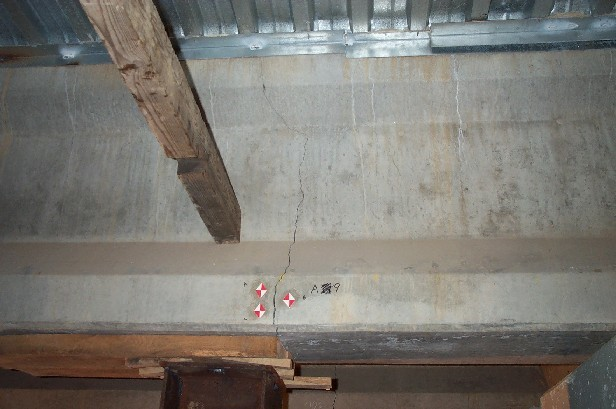
\includegraphics[height=4.8cm]{cracks-near-supports.jpg}
    % \caption{Cracks near girder supports}
    \caption{梁支承附近开裂}
    \label{fig:cracks-near-supports}
  \end{minipage}%
  \begin{minipage}{0.5\linewidth}\centering
    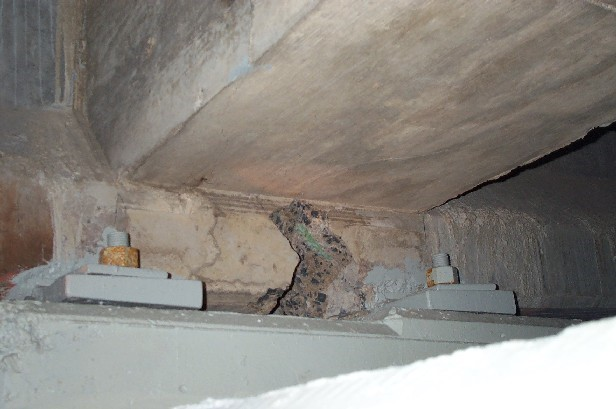
\includegraphics[height=4.8cm]{cracks-spall-diaphragm.jpg}
    % \caption{Crack and spall at diaphragm over pier support}
    \caption{桥墩支承的横隔梁的裂纹和剥落}
    \label{fig:cracks-spall-diaphragm}
  \end{minipage}
\end{figure}

\bigskip 
Because of the uncertainty associated with calculations of positive continuity moments resulting from the variability of the creep and shrinkage effects, temperature gradient, differential coefficient of expansion effects, locked-in heat of hydration effects, settlement, and cracking, calculations to determine restraint moments are complex and probably unreliable. Therefore, in order to eliminate the need to attempt to calculate restraint moments and to simplify the design, the following recommendations for positive moment connections were developed based on the work in the NCHRP projects (Oesterle et at. 1989; Mirmiran et al. 2001; Miller et al. 2004), the FHWA jointless bridge project (Oesterle et al. 2004a, 2004b) and on the Fourth Edition of the LRFD Specifications \cite{aashto2007l}:

\emph{Option 1.} Positive moment connection reinforcement at the piers should not be provided. This approach prevents the development of significant positive restraint moments in the pier diaphragms (and eliminates constructability issues with the overlapping reinforcement). The girders should be analyzed as simply supported for dead plus live loads at service levels. This is allowed by LRFD Specifications Article 5.14.1.4.1; eliminates the requirement to calculate restraint moments (without the need to age girders prior to construction); and, as stated in the commentary of the LRFD Specifications, has been used successfully by several state DOTs.

\emph{Option 2}. If positive moment connections are used to improve structural integrity and to provide some crack control, as recommended in the commentary of LRFD Specifications Article 5.14.1.4.1, it is suggested that the positive moment capacity, φMn, be limited to the minimum moment of 0.6 Mcr recommended in the LRFD Specifications. Note that Mcr should be determined using the properties of the diaphragm concrete. If additional reinforcement is used to increase crack control, the upper limit recommended by the LRFD Specifications of φMn = 1.2 Mcr should not be exceeded. To eliminate the need for calculation of restraint moments, the girders should be analyzed as simply supported for dead plus live loads at service levels as allowed by LRFD Specifications Article 5.14.1.4.1. However, positive restraint moments are likely to occur. In spite of this, additional stresses in the girders due to positive restraint moment can be minimized by limiting the capacity of the connection φMn so that the connection acts as a fuse to yield prior to development of detrimental stresses. Therefore, the girder service load stresses should be checked along the length of the girder under simple supported dead and live loads plus φMn of the positive moment connections superimposed on the spans, such that the allowable tensile stress in the bottom of the beam of 0.19 f c' , ksi, (6 f c' , psi) is not exceeded. Particular attention should be paid to the region of termination of the positive moment steel if mild reinforcement is used for the connection.

\bigskip
For both options 1 and 2, the girder/diaphragm interface should consider details to allow relative movement between the bottom of the girder and diaphragm concrete for girders partially embedded in the diaphragm concrete. For the exterior surface of fascia girders, providing a sealed crack control joint at the beam-to-diaphragm interface should be considered.

Negative moment reinforcement should be provided over the supports, and diaphragm concrete should be provided between the ends of the girder bottom flanges. Negative restraint moments may develop, for example when the deck and diaphragms are cast when the concrete girders are older. However, parametric studies carried out in the FHWA jointless bridge project indicate that, with high restraint moments, cracking occurs in the deck and sufficient moment redistribution occurs to prevent the deck reinforcement from becoming overstressed. Therefore, restraint moments do not have to be calculated. Negative moment reinforcement in the deck can be designed for applied dead and live load moments calculated based on uncracked section properties. It can be assumed tht the girder is simply supported for dead load and fully continuous for live and superimposed dead loads, because of the parapets, barrier walls, wear surface, etc.. Since the deck in the negative moment region is considered reinforced concrete, the negative moment connection is only designed for strength limit states.


% \subsection{Restraint Moments in Composite Steel Bridge Girders}
\subsection{组合钢梁桥中的约束力矩}
% Temperature gradients and differential coefficients of thermal expansion in continuous composite steel beams produce both positive and negative restraint moments, while the shrinkage of deck concrete and the heat of hydration locked-in strains produce negative restraint moments. Deck slab cracking partially relieves negative restraint moments.
连续组合钢梁中的温度梯度和微分热膨胀系数会产生正负约束力矩,而桥面板混凝土的收缩和水化热锁定应变会产生负约束力矩。 甲板板开裂部分缓解了负约束力矩。

% The parametric studies in the FHWA jointless bridge project indicate that stresses in both the concrete deck slab and steel beams are not excessive under the combination of dead and live load forces combined with positive restraint moments. Therefore, explicit calculations considering positive restraint moments are not necessary.
FHWA 无缝桥项目中的参数研究表明,在恒载和活载力以及正约束力矩的组合下,混凝土桥面板和钢梁中的应力都不会过大。 因此,不需要考虑正约束力矩的显式计算。

% moments are high, deck cracking results in redistribution and calculated stresses are not excessive. However, analyses also included the effects of a negative temperature gradient, which produces negative restraint moments, combined with dead and live load and restraint of longitudinal expansion provided by passive pressure in backfill and the lateral force in the piles of integral abutments. These analyses indicated that, under certain circumstances, calculated compressive stresses in the bottom flange of the steel beams near interior supports may be excessive, even after allowance for redistribution of the stresses because of deck cracking. Based on the parametric studies, the combination of loads described above may become critical for larger beam spacing. Calculations indicate that, for stringer spacing equal to or greater than 7 ft for A36 beams, and 9 ft for A572, Grade 50 beams, an explicit check of the effects of the combined load effects of dead and live loads, negative temperature gradient, and restraint of longitudinal expansion may be required to check for lateral torsional buckling of the bottom flange near interior supports.
力矩很高,甲板开裂会导致重新分配,计算出的应力不会过大。 然而,分析还包括产生负约束力矩的负温度梯度的影响,结合恒荷载和活荷载以及回填中的被动压力和整体桥台桩中的侧向力提供的纵向膨胀约束。 这些分析表明,在某些情况下,计算得出的靠近内部支撑的钢梁底部翼缘的压应力可能过大,即使考虑到由于甲板开裂引起的应力重新分布后也是如此。 根据参数研究,上述载荷组合可能对较大的梁间距至关重要。 计算表明,对于 A36 梁的纵梁间距等于或大于 7 英尺,A572 的纵梁间距等于或大于 9 英尺,50 级梁,明确检查恒载和活载、负温度梯度和 可能需要限制纵向膨胀以检查靠近内部支撑的底部法兰的横向扭转屈曲。
